\section{Predicate Class Reference}
\label{class_predicate}\index{Predicate@{Predicate}}
Mother abstract functor representing a predicate.  


{\tt \#include $<$Predicate.hxx$>$}

Inheritance diagram for Predicate::\begin{figure}[H]
\begin{center}
\leavevmode
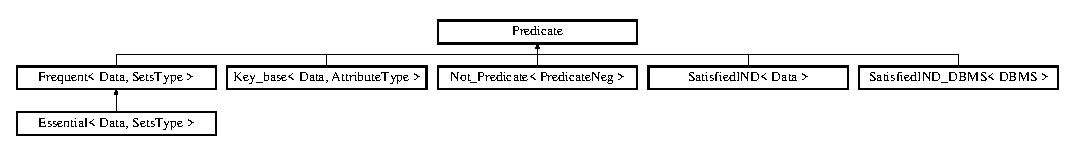
\includegraphics[height=1.6cm]{class_predicate}
\end{center}
\end{figure}
\subsection*{Public Member Functions}
\begin{CompactItemize}
\item 
{\bf Predicate} ()\label{class_predicate_50088fcbd7632e6be3b2df62441535af}

\begin{CompactList}\small\item\em Constructor. \item\end{CompactList}\item 
virtual {\bf $\sim$Predicate} ()\label{class_predicate_91060d92c2f251fd3b0072a3c08f3911}

\begin{CompactList}\small\item\em Destructor. \item\end{CompactList}\item 
template$<$class Iterator, class Measure$>$ bool {\bf operator()} (Iterator word\-It, Measure \&mes\-Cand)
\begin{CompactList}\small\item\em Operator that test if a word of the language is interesting wrt predicate or not. \item\end{CompactList}\item 
template$<$class Cand\_\-Data\-Struct, class f$>$ void {\bf pre\-Processing} (Cand\_\-Data\-Struct \&cand, f word\-To\-Set)
\begin{CompactList}\small\item\em Function used to do some pre processing operations before testing the candidates generated. \item\end{CompactList}\item 
template$<$class Cand\_\-Data\-Struct, class f$>$ void {\bf post\-Processing} (Cand\_\-Data\-Struct \&cand, f word\-To\-Set)
\begin{CompactList}\small\item\em Function used to do some post processing operations after testing the candidates generated. \item\end{CompactList}\end{CompactItemize}


\subsection{Detailed Description}
Mother abstract functor representing a predicate. 

This functor test if an itemset is interesting wrt the predicate. The template parameter Iterator is an iterator on a candidate. 



\subsection{Member Function Documentation}
\index{Predicate@{Predicate}!operator()@{operator()}}
\index{operator()@{operator()}!Predicate@{Predicate}}
\subsubsection{\setlength{\rightskip}{0pt plus 5cm}template$<$class Iterator, class Measure$>$ bool Predicate::operator() (Iterator {\em word\-It}, Measure \& {\em mes\-Cand})\hspace{0.3cm}{\tt  [inline]}}\label{class_predicate_6fb1a75dba2268f75738f335f403e46c}


Operator that test if a word of the language is interesting wrt predicate or not. 

\begin{Desc}
\item[Parameters:]
\begin{description}
\item[{\em word\-It}]iterator on the word to test. \end{description}
\end{Desc}


Reimplemented in {\bf Not\_\-Predicate$<$ Predicate\-Neg $>$} {\rm (p.\,\pageref{class_not___predicate_c4dd938a356c8476e50806158069d169})}, {\bf Satisfied\-IND$<$ Data $>$} {\rm (p.\,\pageref{class_satisfied_i_n_d_bbf69fd5dfbf71f8e7f0685b80551c6d})}, {\bf Satisfied\-IND\_\-DBMS$<$ DBMS $>$} {\rm (p.\,\pageref{class_satisfied_i_n_d___d_b_m_s_10cb098e49804f3de10b20c1d3317814})}, {\bf Essential$<$ Data, Sets\-Type $>$} {\rm (p.\,\pageref{class_essential_e6a89fa2543fe441619066b0f4f6323b})}, {\bf Frequent$<$ Data, Sets\-Type $>$} {\rm (p.\,\pageref{class_frequent_82e02ab1cf1749ea52e9603dc06a5d15})}, and {\bf Key\_\-base$<$ Data, Attribute\-Type $>$} {\rm (p.\,\pageref{class_key__base_27f6933ca653e959cea1332231c1ee8a})}.\index{Predicate@{Predicate}!postProcessing@{postProcessing}}
\index{postProcessing@{postProcessing}!Predicate@{Predicate}}
\subsubsection{\setlength{\rightskip}{0pt plus 5cm}template$<$class Cand\_\-Data\-Struct, class f$>$ void Predicate::post\-Processing (Cand\_\-Data\-Struct \& {\em cand}, f {\em word\-To\-Set})\hspace{0.3cm}{\tt  [inline]}}\label{class_predicate_49f7acb334fac851a26a4d1aecc64571}


Function used to do some post processing operations after testing the candidates generated. 

\begin{Desc}
\item[Parameters:]
\begin{description}
\item[{\em cand}]container of words of the language. \end{description}
\end{Desc}


Reimplemented in {\bf Frequent$<$ Data, Sets\-Type $>$} {\rm (p.\,\pageref{class_frequent_ff29167beb828195c34e10881abb2f74})}.\index{Predicate@{Predicate}!preProcessing@{preProcessing}}
\index{preProcessing@{preProcessing}!Predicate@{Predicate}}
\subsubsection{\setlength{\rightskip}{0pt plus 5cm}template$<$class Cand\_\-Data\-Struct, class f$>$ void Predicate::pre\-Processing (Cand\_\-Data\-Struct \& {\em cand}, f {\em word\-To\-Set})\hspace{0.3cm}{\tt  [inline]}}\label{class_predicate_8ee59d790e9b46e5e0555dbeb5b91f95}


Function used to do some pre processing operations before testing the candidates generated. 

\begin{Desc}
\item[Parameters:]
\begin{description}
\item[{\em cand}]container of words of the language. \end{description}
\end{Desc}


Reimplemented in {\bf Frequent$<$ Data, Sets\-Type $>$} {\rm (p.\,\pageref{class_frequent_236bb06ebfac503436c8a25a8507b467})}.

The documentation for this class was generated from the following file:\begin{CompactItemize}
\item 
F:/i\-Zi/problems/Predicate.hxx\end{CompactItemize}
